\documentclass[11pt]{article}
\usepackage{amsmath}
\usepackage{amssymb}
\usepackage{graphicx}
\usepackage{booktabs}
\usepackage{geometry}
\usepackage{tikz}
\usepackage{pgfplots}
\usepackage{tabularx}
\usepackage{url}
\usepackage{hyperref}
\makeatletter\g@addto@macro\UrlBreaks{\do\-\do\_}\makeatother
\pgfplotsset{compat=1.17}
\usetikzlibrary{arrows.meta,positioning}
\geometry{margin=1in}

\title{Pruned multi-angle QAOA does not reach the 35-CNOT thermofield-double anchor at matched cost: five certified sparse-SYK instances at $\beta = 3$}
\author{Gyalpo Dongo \and Sebastian Alberdi}
\date{22 September 2026}

\begin{document}
\maketitle

\begin{abstract}
Preparing the thermofield double (TFD) state is the entry cost of sparse Sachdev-Ye-Kitaev (SYK) wormhole and scrambling experiments, a cost dominated by two-qubit gates. A recent preprint proposes preparing it with a multi-angle QAOA ansatz reduced by sequential angle pruning (SAP) and its ordered variant (OSAP), and does not include a comparison with a 35-CNOT block. That fixed hardware-efficient block is the authors' own hardware TFD circuit, and they told us it transpiles to 35 CZ on ibm\_marrakesh. We test the preprint's pruning against that block on five certified sparse-SYK instances at inverse temperature $\beta = 3$, each on eight qubits in its own Jordan-Wigner map, with the preprint's pruning algorithms, optimizer budgets and candidate-pool size and two disclosed deviations (two weight-2 mixer strings treated as prunable blocks; a pre-registered small-angle start on four instances). Here we show a clear null on four instances and a borderline case on the fifth. On Rows 42, 48, 32 and 30, pruned ma-QAOA at 35 two-qubit gates falls short of the block by 0.06 to 0.14 under every definition we checked (routed or logical axis; converged, best-of-6 or contract anchor). On Eq. 11, OSAP reaches $F = 0.925$ at 35 logical CNOTs, above the contract's sealed anchor (0.923) and 0.014 below the converged anchor (0.938), but that circuit routes to 43 CZ, and within 35 routed CZ the best is 0.904. The pre-registered decision rule (routed axis, converged anchor, 0.02 margin) returns NULL on all five instances; on Eq. 11 that verdict depends on those axis and anchor choices, and under the campaign's original frozen contract (logical axis, sealed anchor) Eq. 11 would not be a null. At $\leq 35$ routed CZ the best fidelities are 0.802 to 0.904 (OSAP) and 0.766 to 0.821 (SAP), against a converged anchor of 0.936 to 0.949. Reaching the converged anchor costs OSAP 93 to 103 logical CNOTs on four instances and 41 on Eq. 11, and OSAP dominates SAP, consistent with the preprint. A by-product favours the block: its converged own-map anchor exceeds the 0.887 to 0.915 of our earlier study, with encoding and fit effort (6 x 800 to 50 x 3000) changed together.
\end{abstract}

\section{Introduction}

The thermofield double state of a Hamiltonian $H$ at inverse temperature $\beta$ is the pure state on two copies of the system whose reduced density matrix on either copy is the thermal state $e^{-\beta H}/Z$. For the Sachdev-Ye-Kitaev (SYK) model \cite{sachdev1993,maldacena2016} it is the object that every traversable-wormhole and scrambling protocol starts from \cite{gao2017,maldacena2018,jafferis2022}: the wormhole teleportation signal is read out of a coupled pair of SYK systems that must first be put into, or close to, their TFD. Sparse SYK models \cite{xu2020,tezuka2023} make this tractable on small registers by keeping only $K$ of the four-fermion terms, which is what puts eight-qubit doubled registers within reach of both exact simulation and near-term devices.

The practical question is not whether the TFD can be prepared but how many two-qubit gates it takes. On superconducting hardware the two-qubit count is the dominant error budget, so a preparation circuit is judged on a fidelity-versus-cost curve rather than on fidelity alone. Two families of preparation circuit compete. The first is hardware-efficient: a fixed, instance-blind entangling topology whose single-qubit rotation angles are fitted per instance, in our case a six-layer block containing exactly 35 CNOTs. The second is physics-shaped: a multi-angle QAOA (ma-QAOA) ansatz \cite{herrman2022,farhi2014} built from the instance's own cost and mixer Hamiltonians, which is expressive but expensive, because each four-body Pauli evolution compiles to a CNOT ladder. A recent preprint by Ashfaq, Byun and Kim \cite{gist2026} closes that gap by pruning: fit the ma-QAOA ansatz to high fidelity, then delete nonlocal blocks one at a time, reoptimizing the surviving angles after each deletion. Their Algorithm 1 (sequential angle pruning, SAP) deletes the smallest-angle block; their Algorithm 2 (ordered SAP, OSAP) tries the $N_C$ smallest-angle blocks and keeps whichever deletion costs least fidelity after reoptimization. The preprint does not compare with a 35-CNOT block. That block is the variational TFD circuit the authors use in their hardware work, and they told us by email that it transpiles to 35 CZ on ibm\_marrakesh (private communication from the authors, 15 September 2026). This paper tests the preprint's pruning against that block. The preprint tests $\beta = 0.1$, 1 and 10 and reports that pruning is most effective at low temperature; $\beta = 3$ is outside the values it tests, and our result says nothing about the other temperatures.

This paper answers one question. On five sparse-SYK instances we had already certified in earlier work \cite{dongo2026instances}, at $\beta = 3$, does pruned ma-QAOA reach the fidelity of the fixed 35-CNOT block at a cost of at most 35 two-qubit gates, the cost of that block after routing to a real coupling map? We ran their algorithms literally, at their optimizer budgets, against an anchor fitted to convergence, with the decision rule written down and committed before the computation ran. The answer is a clear no on four instances under every cost axis and anchor we checked. On Eq. 11 it is borderline: the pre-registered rule returns no, but at 35 logical CNOTs OSAP nearly matches the block, and the verdict there rests on the routed axis and the converged anchor. The crossing point is measured rather than estimated. We also report a result that favours the block: fitted to convergence in each instance's own Jordan-Wigner map, it is substantially better than in our earlier certified-instance study, which raises the bar that any pruned ansatz has to clear.

The contribution is a boundary, not a method. We state where the pruned ansatz sits on the fidelity-versus-cost curve, what it would cost to reach the anchor, and exactly which assumptions the boundary depends on.

\section{Setting}

\subsection{Instances, encoding and targets}

The five instances are the certified binary sparse-SYK instances of our earlier certified-instance study \cite{dongo2026instances}: Row 42 (INST-A, the primary instance), Rows 48, 32 and 30 (INST-B, INST-C, INST-D), and the instance of Eq.~(11) of Byun, Kim and Lee \cite{byun2026wormhole} (``Eq. 11'', INST-E). Each has $N = 8$ Majorana fermions per side and $K$ four-body terms with signs $\pm 1$: $K = 12$, 11, 13, 12 and 10 (Row 42, 48, 32, 30, Eq. 11), with coupling scale $J_c = \sqrt{2}/\sqrt{K} = 0.4082$, 0.4264, 0.3922, 0.4082 and 0.4472. This is the preprint's own normalization ($J = \sqrt{2}$, binary coefficient $J/\sqrt{K}$), so $\beta$ needs no rescaling. The doubled system is encoded on eight qubits in the shared-register convention of the preprint's Eq. 5, so the left and right SYK copies live on the same eight qubits rather than on four each.

The reference state $|I\rangle$ is the ground state of the left-right coupling $H_{\mathrm{int}}$. In this encoding it factorizes as a Bell-like pair on qubits 0 and 1 tensored with $|0\rangle$ on qubits 2 through 7, so it is prepared from $|0\rangle^{\otimes 8}$ by the verified one-CX circuit \texttt{x(1) h(0) cx(0,1) s(0)}, whose fidelity to $|I\rangle$ is 1 in every instance map. That single CX is counted in every cost we report. The target is
\begin{equation}
|\mathrm{TFD}_\beta\rangle \;=\; \mathcal{N}\, e^{-\beta H_{\mathrm{tot}}/4}\,|I\rangle, \qquad H_{\mathrm{tot}} = H_L + H_R, \qquad \beta = 3,
\end{equation}
with $\mathcal{N}$ a normalization, built by the sealed target builder of our earlier certified-instance study so that the convention is reused verbatim rather than re-derived.

One encoding choice matters enough to state up front. Each instance carries its own Jordan-Wigner map \cite{jordanwigner1928}, the map its protocol circuit actually runs in, and targets here are built in that map. The default-map and instance-map TFDs are the same physical state written in two qubit encodings; their raw overlap of only 0.52 to 0.59 reflects the qubit relabeling, not a different state. SAP and OSAP fidelities do not depend on the map: the ma-QAOA ansatz is the same circuit family in every map, because each Pauli label differs at most by a sign that is absorbed into its angle (checked to $2\times 10^{-17}$ with angles mapped by that sign). The map does change the routed cost, and the fitted fidelity of the fixed 35-CNOT block, which is a qubit-level ansatz. That is why the instance map, where the protocol circuit runs, is the right one for comparing costs. An independent reconstruction of the targets from the paper's equations matched every stored target to fidelity $1 - 10^{-12}$ (repro package: \path{workspace/convention_check.py}, \path{workspace/director-convention-check-2026-09-22.json}); the Hamiltonian's overall sign is pinned by the hardware paper's published teleportation peak (0.374 at $t_1 = 2.3$ is reproduced; the opposite sign gives 0.275 at $t_1 = 2.0$). Every fidelity in Sections 4.1 to 4.4 is an instance-map fidelity unless the table says otherwise.

\subsection{Two cost axes}

We report two costs for every circuit. The \emph{logical} cost counts two-qubit gates in the emitted gate list, with \texttt{cx} and \texttt{cz} costing 1 and \texttt{rzz}, \texttt{rxx}, \texttt{ryy} costing 2, so an evolution $e^{-i\theta P/2}$ of a weight-$w$ Pauli string costs $2(w-1)$ (the preprint's Eq. 19 CNOT ladder). The \emph{routed} cost is the two-qubit count after transpiling the circuit to a real coupling map: FakeMarrakesh, optimization level 3, best of eleven pinned seeds. Logical savings do not automatically survive routing, and routed cost is the axis a device pays. The preprint authors' own cost figure for the block (35 CZ) is a routed count on ibm\_marrakesh, so the decision rule below is written on the routed axis. The logical count is reported alongside it because the campaign's frozen contract defined the null there.

\section{Methods}

\subsection{Ansatz and pruning, taken literally}

The ansatz, the pruning algorithms and the optimizer budgets follow the preprint, with two deliberate deviations: the two weight-2 mixer strings on qubits 0 and 1 are treated as prunable nonlocal blocks, and pruning starts from the small-angle initialization set B on four of five instances, per the pre-registered rule below.

The ansatz is the preprint's Eq. 18. With $p$ layers,
\begin{equation}
|\psi\rangle \;=\; \prod_{l=1}^{p} \Big[\prod_{\mu} e^{-i t^{M}_{l\mu} P^{M}_{\mu}}\Big]\Big[\prod_{\nu} e^{-i t^{C}_{l\nu} P^{C}_{\nu}}\Big]\,|I\rangle ,
\end{equation}
one independent angle per Pauli string per layer. The cost strings $P^C$ are the $2K$ Pauli strings of $H_L + H_R$ in the instance's term order, left then right; the mixer strings $P^M$ are the $N = 8$ strings of $H_{\mathrm{int}}$ in $j$ order. Within a layer the cost strings act first.

A \emph{nonlocal block} is any evolution whose Pauli weight is at least 2, which is every cost string plus, in this encoding, the two weight-2 mixer strings on qubits 0 and 1. Weight-1 evolutions are free on the two-qubit axis and are never pruned. SAP removes the active nonlocal block of smallest $|t|$, with $t$ wrapped to $(-\pi,\pi]$, then reoptimizes. OSAP with $N_C = 10$ forms a candidate pool from the ten smallest-$|t|$ active blocks, tries each deletion with a reoptimization, and keeps the one with the lowest loss. Both run down to zero nonlocal blocks, so the full curve is measured rather than truncated at a budget.

The objective is $L = 1 - |\langle \mathrm{TFD}|\psi\rangle|^2$ with an analytic adjoint gradient, minimized with L-BFGS-B \cite{byrd1995,scipy2020} at \texttt{ftol} 0 and \texttt{gtol} $10^{-10}$. The initial fit sweeps $p = 3,4,\dots,8$ and stops at the first $p$ whose best fidelity reaches 0.9999, with 5 initializations per $p$ at 3000 iterations. Two initialization sets are run and both are reported: set A, the literal reading of ``random'', $t \sim U(-\pi,\pi)$; and set B, a labelled sensitivity arm, $t \sim U(-0.1,0.1)$. Pruning starts from whichever set reaches 0.9999 at the smaller $p$, with ties going to set A. Pruning rounds warm-start from the current angles in a box $[t-\pi, t+\pi]$ at 300 iterations, with no random restarts inside the loop, which is the preprint's budget.

A separate post-hoc polish never feeds selection: for each instance and algorithm, the highest-fidelity point at 35 routed CZ or less is refitted on its fixed structure from 6 initializations at 800 iterations.

\subsection{The anchor}

The comparison target is the fixed hardware-efficient block: eight Hadamards, then six layers of per-qubit $R_z R_x$ rotations interleaved with five linear CNOT chains, 35 CNOTs and 96 angles. Its anchor fidelity $F_{35}^{*}$ is the block fitted to each instance-map target at the best of 50 initializations times 3000 L-BFGS-B iterations. Its routed cost $A_{35}$ is measured on FakeMarrakesh, not assumed.

A stronger anchor makes a null easier to obtain, so a converged anchor alone would favour our conclusion. The paper therefore also tests the null against the weak anchor, the unconverged best-of-6 instance-map fit, reported alongside the converged one (Section 4.2).

\subsection{Harness protocol}

The campaign ran in an autoresearch harness whose rules are mechanical. A hypothesis is pre-registered with its prediction, its falsifier and its kill threshold before any implementation; an adversarial challenge gate reads the hypothesis before a coder implements it; a blinded scorer simulates the submitted gate list itself, from $|0\rangle^{\otimes 8}$, against a sealed target, recomputes both fidelity and cost, and discards everything the candidate reports about its own performance; a candidate is promoted only when the blinded score improves on the incumbent. The scored quantity in this campaign is
\begin{equation}
s_i \;=\; 1000 \cdot \max\!\left(0,\; F_{35,i} - F_i\right) \;+\; C_{2,i}, \qquad \mathrm{score} = \tfrac{1}{5}\sum_i s_i ,
\label{eq:score}
\end{equation}
with the contract's sealed per-instance $F_{35,i}$, so that cost can never be bought by giving up fidelity and, above the anchor, the objective is simply two-qubit cost.

The result in Sections 4.1 to 4.4 is a pre-registered computation run outside the scored loop, not a ledger trial verdict. Its decision rule was written down before it ran (repro package: \path{workspace/PREREG-maqaoa-2026-09-22.md}); the code that ran it is in the repro package (\path{workspace/maqaoa_prune.py}); and the 155 stored points (every point at logical cost 70 or less, every tenth pruning round, and both endpoints) were re-verified through the sealed scorer's own gate-list simulator. The crossing values at higher cost come from the optimizer's own simulator, which agrees with the independent gate-list simulation on all 155 stored points to $10^{-13}$. We say this plainly because the harness's own rule is that nothing self-reported enters a ledger: these numbers are verified computations run under a committed pre-registration, and they are labelled as such throughout.

\subsection{Verification}

Three checks had to pass before any number here was reported. First, each of the 155 stored points (every point at logical cost 70 or less, every tenth pruning round, and both endpoints) was emitted as a scorer-format gate list and re-simulated by the sealed scorer's simulator from $|0\rangle^{\otimes 8}$ against the sealed instance-map target, with agreement required to $10^{-8}$ and the gate list's CX count required to equal the recorded logical cost. Second, the analytic gradient had to pass a central-difference check below $10^{-6}$ at a random $p = 3$ point on each instance. Third, on one circuit the Qiskit statevector before transpilation had to match the gate-list simulation to $10^{-8}$ up to global phase \cite{qiskit2024}. All three passed.

All fidelities in this paper are exact noiseless statevector overlaps on the 256-dimensional doubled register. No noise model, no sampling and no device execution enters any number here; routing enters only as a gate count.

\subsection{Validation against the preprint's published numbers}

Before trusting a null, we checked that our implementation reproduces the preprint's own results. The check was pre-registered, with agreement criteria committed before it ran (repro package: \path{workspace/reproduce_preprint.py}, \path{workspace/director-preprint-reproduction-2026-09-22.json}). The same code that produced Section 4, run on 20 fresh binary sparse $N = 8$, $K = 10$ instances in the preprint's own encoding, reproduces its published averages (Table~\ref{tab:repro}, which lists every pre-registered comparison). Two independent 20-sample means were pre-registered to agree when they differ by at most $2\sigma\sqrt{2/20}$, where $\sigma$ is the preprint's reported realization-to-realization spread. The Table I agreement holds only with small initial angles, $U(-0.1, 0.1)$: the full-range $U(-\pi,\pi)$ misses Table I at $\beta = 10$ (0.974 against 0.988, outside the 0.0057 tolerance), which is why the small-angle set is the one that reproduces the preprint; the pre-registered T1 test requires one initialization set to pass. The largest discrepancy is SAP at $\beta = 10$, $S = 19$ (ours 0.896 against their 0.869); it is within the pre-registered tolerance (0.045) because their SAP spread at $\beta = 10$ is large ($\sigma = 0.072$), ours is higher rather than lower, and the OSAP row at the same point agrees to $5\times 10^{-5}$. Every pre-registered agreement criterion passed. The reaching depth at $\beta = 10$ runs up to one layer deeper than the preprint reports on 4 of 20 instances. Otherwise the averages agree within the stated tolerances, which makes an implementation error an unlikely explanation for the null in Section 4.

\begin{table}[t]
\centering
\small
\resizebox{\textwidth}{!}{\begin{tabular}{lllccc}
\toprule
Test & Preprint table & Quantity & Ours & Preprint & Tolerance \\
\midrule
T1 & Table I ($\beta = 0.1$, $p = 3$) & mean $F$, set A / set B & 1.000000 / 1.000000 & 1.000000 & ours $\geq 0.9999$ \\
T1 & Table I ($\beta = 1$, $p = 3$) & mean $F$, set A / set B & 0.999981 / 0.999999 & 0.999999 & ours $\geq 0.9999$ \\
T1 & Table I ($\beta = 10$, $p = 3$) & mean $F$, set A & 0.9741 (miss) & 0.9879 & 0.0057 \\
T1 & Table I ($\beta = 10$, $p = 3$) & mean $F$, set B & 0.9876 & 0.9879 & 0.0057 \\
T2 & reaching $p$ ($\beta = 10$), set B & range & 4 to 8 & 4 to 7 & overlap \\
T2 & reaching $p$ ($\beta = 10$), set A & reached by $p = 8$ & 1 of 20 & 4 to 7 & (reported) \\
T3 & Table V ($\beta = 0.1$, $S = 1$) & SAP mean $F$ & 0.999719 & 0.999719 & $1\times 10^{-4}$ \\
T3 & Table V ($\beta = 0.1$, $S = 1$) & OSAP mean $F$ & 0.999719 & 0.999719 & $1\times 10^{-4}$ \\
T3 & Table V ($\beta = 1$, $S = 1$) & SAP mean $F$ & 0.972675 & 0.972688 & $4.0\times 10^{-4}$ \\
T3 & Table V ($\beta = 1$, $S = 1$) & OSAP mean $F$ & 0.972888 & 0.972709 & $4.2\times 10^{-4}$ \\
T3 & Table V ($\beta = 10$, $S = 19$) & SAP mean $F$ & 0.8959 & 0.8687 & 0.0453 \\
T3 & Table V ($\beta = 10$, $S = 19$) & OSAP mean $F$ & 0.9574 & 0.9574 & 0.0128 \\
T4 & Table III ($\beta = 10$, $F \approx 0.98$) & SAP blocks / two-qubit gates & 31.4 / 283 & 31 / 292 & 4.4 / 43.6 \\
T4 & Table III ($\beta = 10$, $F \approx 0.98$) & OSAP blocks / two-qubit gates & 24.9 / 224 & 25 / 229 & 3.2 / 38.6 \\
\bottomrule
\end{tabular}}
\caption{Every pre-registered comparison of our SAP/OSAP implementation against the preprint's published averages, on 20 fresh instances in the preprint's encoding. Tolerances are $2\sigma\sqrt{2/20}$ from the preprint's reported spread $\sigma$, except the $\beta = 0.1$ and 1 rows of T1 (an absolute floor) and T2 (range overlap). T1 passes if either initialization set passes; set A misses at $\beta = 10$ and set B passes. T2 is reported per initialization set: with set B all 20 instances reach $F \geq 0.9999$ by $p = 8$ ($p = 4$: 1, $p = 6$: 5, $p = 7$: 10, $p = 8$: 4), so 4 of 20 need one layer more than the preprint's maximum; with set A, 19 of 20 do not reach 0.9999 by $p = 8$ and plateau at 0.998 to 0.999.}
\label{tab:repro}
\end{table}

\begin{figure}[t]
\centering
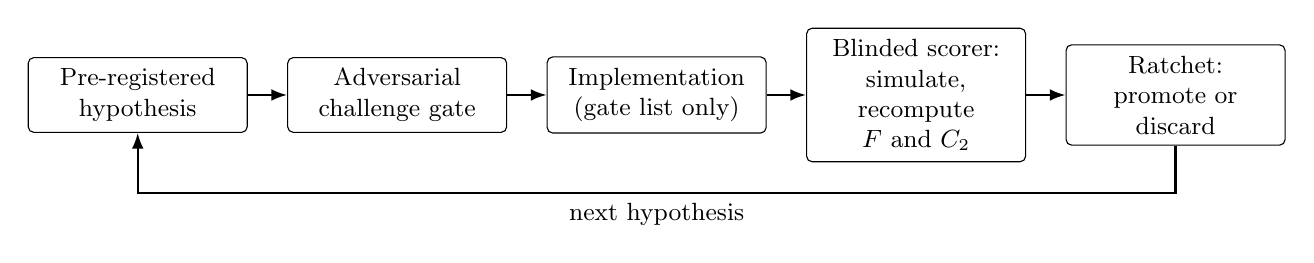
\begin{tikzpicture}[
  node distance=5mm,
  box/.style={draw, rounded corners=2pt, align=center, font=\small, inner sep=4pt, minimum height=9mm, text width=25mm},
  arr/.style={-{Latex[length=2mm]}, thick}
]
\node[box] (h) {Pre-registered\\hypothesis};
\node[box, right=of h] (c) {Adversarial\\challenge gate};
\node[box, right=of c] (i) {Implementation\\(gate list only)};
\node[box, right=of i] (s) {Blinded scorer:\\simulate, recompute\\$F$ and $C_2$};
\node[box, right=of s] (r) {Ratchet:\\promote or discard};
\draw[arr] (h) -- (c);
\draw[arr] (c) -- (i);
\draw[arr] (i) -- (s);
\draw[arr] (s) -- (r);
\draw[arr] (r.south) -- ++(0,-6mm) -| node[pos=0.25, below, font=\small] {next hypothesis} (h.south);
\end{tikzpicture}
\caption{The harness loop for this campaign. Nothing a candidate reports about itself is read: the scorer simulates the submitted gate list from $|0\rangle^{\otimes 8}$, recomputes the fidelity against a sealed target and recounts the two-qubit cost, and only that verdict can promote a candidate. The pruning results of Section 4 were produced by a pre-registered computation run outside the scored loop and then pushed back through the same scorer simulator for verification.}
\label{fig:loop}
\end{figure}

\section{Results}

\subsection{Reachability: the unpruned ansatz gets there, expensively}

Pruning a ceiling that does not exist would be uninterpretable, so the first pre-registered gate was reachability: does the unpruned ma-QAOA ansatz reach $F \geq 0.9999$ by $p = 8$? Set B, small initial angles, reaches $F \geq 0.9999$ at $p = 3$ on all five instances; set A, the literal $U(-\pi,\pi)$ reading, reaches it at $p = 3$ on Row 48 (INST-B), at $p = 8$ on Rows 42, 32 and 30 (INST-A, INST-C, INST-D), and never by $p = 8$ on Eq. 11 (INST-E) (Table~\ref{tab:reach}). Under the pre-registered rule, pruning therefore started from set B on four instances and from set A on INST-B, where both sets reached $p = 3$ and the tie went to A.

The preprint does not state its initialization. Small initial angles reproduce its Table I, and at $\beta = 3$ the choice matters.

The cost of that reachable point is the reason pruning is needed at all: the converged unpruned circuits cost 499 to 817 logical CNOTs, 14 to 23 times the 35 CNOTs of the block.

\begin{table}[t]
\centering
\begin{tabular}{llccccr}
\toprule
Instance & Row & Set A $p$ & Set B $p$ & Pruned from & Full $F$ & Full logical CNOTs \\
\midrule
INST-A & Row 42 & 8 & 3 & B ($p=3$) & 0.999942 & 751 \\
INST-B & Row 48 & 3 & 3 & A ($p=3$) & 0.999906 & 673 \\
INST-C & Row 32 & 8 & 3 & B ($p=3$) & 0.999924 & 817 \\
INST-D & Row 30 & 8 & 3 & B ($p=3$) & 0.999935 & 763 \\
INST-E & Eq. 11 & none & 3 & B ($p=3$) & 0.999928 & 499 \\
\bottomrule
\end{tabular}
\caption[]{Reachability of the unpruned ma-QAOA ansatz (repro package: \path{workspace/director-maqaoa-trajectories-2026-09-22.json} and \path{workspace/director-maqaoa-crossing-2026-09-22.json}). ``Set A/B $p$'' is the first layer count whose best of 5 fits reaches $F \geq 0.9999$; ``none'' means it was not reached by $p = 8$. ``Full $F$'' and ``Full logical CNOTs'' describe the converged unpruned circuit that pruning starts from, including the one CX that prepares $|I\rangle$.}
\label{tab:reach}
\end{table}

\subsection{At matched cost the pruned ansatz does not reach the anchor}

The routed cost of the standalone 35-CNOT block is $A_{35} = 35$ CZ, identical on all eleven pinned transpiler seeds, which matches the 35 CZ the authors reported to us for their ibm\_marrakesh transpile. The matched-cost budget is therefore 35 routed CZ.

Table~\ref{tab:null} gives the result under the pre-registered rule. On every instance, the best SAP or OSAP point inside that budget falls short of the converged anchor by more than the pre-registered 0.02 margin. The pre-registered post-hoc polish ($6 \times 800$) left the best point unchanged to $10^{-14}$ in 9 of 10 instance-algorithm pairs, and moved Row 48 SAP from 0.8158 to 0.8188 (repro package: \path{workspace/director-maqaoa-decision-2026-09-22.json}), so it changes no verdict. The pre-registered rule declares NULL per instance when that holds, and NULL for the campaign when it holds on all five. It does, and the campaign closes as QUESTION-STATUS with the crossing measured. On Eq. 11, however, this verdict depends on the axis and anchor choices of the second pre-registration (Table~\ref{tab:matrix}). At exactly 35 logical CNOTs OSAP reaches $F = 0.925$ there, above the contract's sealed anchor (0.923) and the best-of-6 instance-map anchor (0.924) and 0.014 below the converged anchor (0.938); that circuit routes to 43 CZ, and within 35 routed CZ the best is 0.904, 0.034 below the converged anchor. The campaign's original frozen contract used the logical axis and the sealed anchor, and under it Eq. 11 would not be a null. On Rows 42, 48, 32 and 30 the shortfall is 0.06 to 0.14 under every combination in Table~\ref{tab:matrix}. The honest summary is a clear null on four instances; on Eq. 11 the pruned ansatz nearly matches the fixed block at 35 logical CNOTs, but not at the same routed cost.

Against the unconverged best-of-6 instance-map anchor (Table~\ref{tab:anchor}), the OSAP margins on INST-A through INST-D are 0.096, 0.067, 0.100 and 0.090, and on Eq. 11 the gap is 0.0200, above the 0.02 margin by $4\times 10^{-5}$ (repro package: \path{workspace/director-null-robustness-2026-09-22.json}). On the routed axis the null therefore holds against the best-of-6 anchor on all five instances, but only marginally on Eq. 11. One confound remains: relative to our earlier certified-instance study \cite{dongo2026instances}, this test changes the encoding (each instance's own map) and the anchor effort (best of 50) together.

OSAP beats SAP at $\leq 35$ CZ and at the crossing on all five instances, which is consistent with the preprint's own claim for the ordered variant.

\paragraph{Post-hoc robustness.} The following probes were run after the verdict and are labelled post-hoc; the verdict is the pre-registered one above (repro package: \path{workspace/director-null-probes-2026-09-22.json}). (i) Matched effort: re-fitting every pruned structure at $\leq 35$ routed CZ from $50 \times 3000$, the anchor's own budget, leaves gaps of 0.034 to 0.14 to $F_{35}^{*}$. (ii) Pruning from $p = 4$ or 5 does not improve on the $p = 3$ start: the best $p = 4$ or 5 point at $\leq 35$ logical CNOTs is 0.898, while the $p = 3$ OSAP trajectory reaches 0.925 at exactly 35 logical CNOTs on Eq. 11. (iii) Of the 155 routed points, none above 35 logical CNOTs routes to $\leq 35$ CZ, so the sparse routing cadence of Section 4.3 missed no point inside the budget.

\begin{table}[t]
\centering
\begin{tabular}{lcccccc}
\toprule
 & & \multicolumn{2}{c}{OSAP} & \multicolumn{2}{c}{SAP} & \\
\cmidrule(lr){3-4}\cmidrule(lr){5-6}
Instance & $F_{35}^{*}$ & best $F$ & routed CZ & best $F$ & routed CZ & Verdict \\
\midrule
INST-A (Row 42) & 0.9424 & 0.8019 & 22 & 0.7661 & 29 & NULL \\
INST-B (Row 48) & 0.9491 & 0.8389 & 34 & 0.8158 & 31 & NULL \\
INST-C (Row 32) & 0.9360 & 0.8364 & 29 & 0.8043 & 29 & NULL \\
INST-D (Row 30) & 0.9464 & 0.8282 & 22 & 0.8052 & 19 & NULL \\
INST-E (Eq. 11) & 0.9383 & 0.9041 & 28 & 0.8207 & 30 & NULL \\
\bottomrule
\end{tabular}
\caption[]{The null (repro package: \path{workspace/director-maqaoa-decision-2026-09-22.json}). For each instance and algorithm, the highest-fidelity pruning point whose routed cost is at most $A_{35} = 35$ CZ, in the algorithm-exact column (warm-start reoptimization only, no random restarts inside the loop). $F_{35}^{*}$ is the 35-CNOT block fitted to convergence in that instance's own Jordan-Wigner map. Every gap exceeds the pre-registered 0.02 margin, so every instance is NULL under the pre-registered rule (routed axis, converged anchor). On INST-E this verdict depends on that axis and anchor choice (Table~\ref{tab:matrix}).}
\label{tab:null}
\end{table}

\begin{table}[t]
\centering
\small
\setlength{\tabcolsep}{4pt}
\begin{tabular}{lcccccc}
\toprule
 & \multicolumn{3}{c}{Best pruned $F$ (OSAP)} & \multicolumn{3}{c}{Block anchor} \\
\cmidrule(lr){2-4}\cmidrule(lr){5-7}
Instance & $\leq 35$ CZ & $\leq 35$ CNOT & its CZ & converged & best-of-6 & sealed \\
\midrule
INST-A (Row 42) & 0.802 & 0.826 & 37 & 0.942 & 0.898 & 0.8955 \\
INST-B (Row 48) & 0.839 & 0.839 & 34 & 0.949 & 0.906 & 0.9164 \\
INST-C (Row 32) & 0.836 & 0.836 & 29 & 0.936 & 0.936 & 0.9011 \\
INST-D (Row 30) & 0.828 & 0.828 & 22 & 0.946 & 0.918 & 0.9228 \\
INST-E (Eq. 11) & 0.904 & 0.925 & 43 & 0.938 & 0.924 & 0.9229 \\
\bottomrule
\end{tabular}
\caption[]{The verdict under every cost axis and anchor we checked (repro package: \path{workspace/director-null-axis-anchor-matrix-2026-09-22.json}). Pruned columns: best OSAP $F$ within 35 routed CZ, best within 35 logical CNOTs, and that point's routed CZ count. ``Converged'' is the best-of-50 instance-map fit $F_{35}^{*}$, ``best-of-6'' the unconverged instance-map fit, ``sealed'' the contract's anchor. On INST-A to INST-D every pruned column is 0.06 to 0.14 below every anchor. On INST-E the best point at $\leq 35$ logical CNOTs clears the sealed and best-of-6 anchors but routes to 43 CZ; within 35 routed CZ it is 0.034 below the converged anchor.}
\label{tab:matrix}
\end{table}

\begin{figure}[t]
\centering
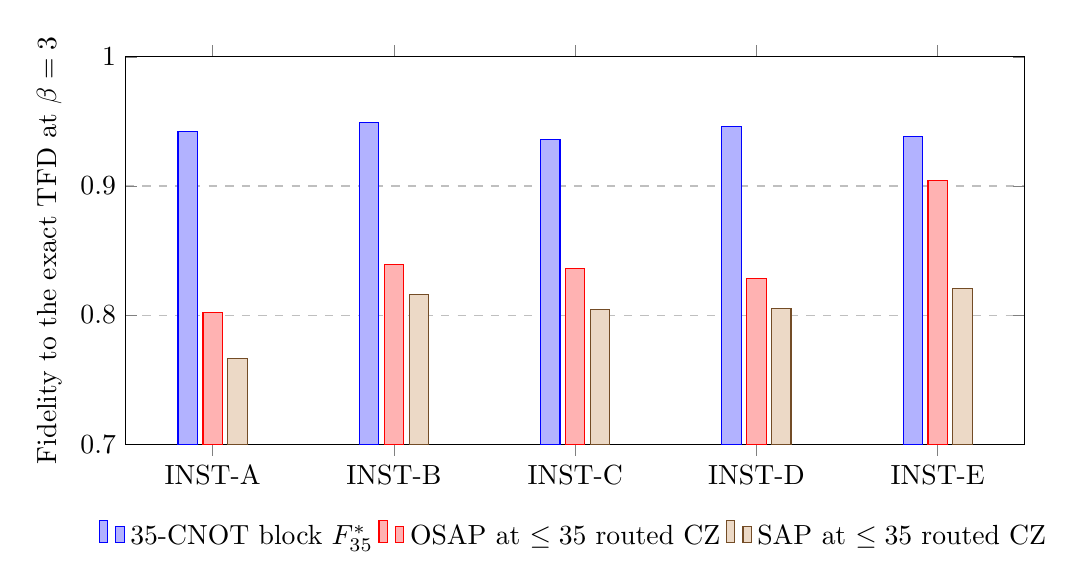
\begin{tikzpicture}
\begin{axis}[
  width=13cm, height=6.5cm,
  ybar, bar width=7pt,
  ymin=0.70, ymax=1.00,
  ylabel={Fidelity to the exact TFD at $\beta=3$},
  symbolic x coords={INST-A,INST-B,INST-C,INST-D,INST-E},
  xtick=data,
  legend style={at={(0.5,-0.18)}, anchor=north, legend columns=3, draw=none},
  ymajorgrids=true, grid style=dashed,
  enlarge x limits=0.12
]
\addplot coordinates {(INST-A,0.9424) (INST-B,0.9491) (INST-C,0.9360) (INST-D,0.9464) (INST-E,0.9383)};
\addplot coordinates {(INST-A,0.8019) (INST-B,0.8389) (INST-C,0.8364) (INST-D,0.8282) (INST-E,0.9041)};
\addplot coordinates {(INST-A,0.7661) (INST-B,0.8158) (INST-C,0.8043) (INST-D,0.8052) (INST-E,0.8207)};
\legend{35-CNOT block $F_{35}^{*}$, OSAP at $\leq 35$ routed CZ, SAP at $\leq 35$ routed CZ}
\end{axis}
\end{tikzpicture}
\caption{At the block's own routed cost, pruned ma-QAOA is behind the block on every instance. Bars are the converged block anchor and the best algorithm-exact SAP and OSAP points with routed cost at most 35 CZ (Table~\ref{tab:null}). The smallest gap, on INST-E, is 0.034, still above the pre-registered 0.02 refutation margin. OSAP is ahead of SAP on all five instances.}
\label{fig:null}
\end{figure}

\subsection{Where the crossing is}

A null at one budget is only half an answer. The pruning curves run all the way down, so the cost at which they do reach the anchor is measurable (Table~\ref{tab:crossing}). On the logical axis OSAP crosses $F_{35}^{*}$ at 93 to 103 CNOTs on four instances and at 41 on INST-E; SAP crosses at 133 to 187. The ordering is the same as at matched cost.

On the routed axis we report an upper bound, not a crossing, in all but two cases, and we state why: routed costs were computed for every point at logical cost 70 or less, for both endpoints, and only for every tenth pruning round in between. The smallest routed cost at which a point with $F \geq F_{35}^{*}$ was observed is therefore an upper bound on the routed crossing wherever the crossing falls in an unrouted stretch. Exact routed crossings exist in exactly two cases: INST-E OSAP at 61 CZ and INST-D SAP at 195 CZ. Elsewhere the routed crossing is only bounded above, for OSAP at $\leq 160$, 139, 149 and 168 CZ on INST-A to INST-D. A reader who wants the exact routed crossings should route the intermediate rounds; the computation is cheap and the data to seed it is in the reproduction package.

The practical reading is that the pruned ansatz is not a cheap substitute for the block on these instances at $\beta = 3$. On the logical axis OSAP buys the anchor fidelity at 2.7 to 2.9 times the block's 35 CNOTs on four of five instances, and at 1.2 times on INST-E; on the routed axis only the upper bounds above are available.

\begin{table}[t]
\centering
\begin{tabular}{lcccc}
\toprule
 & \multicolumn{2}{c}{OSAP} & \multicolumn{2}{c}{SAP} \\
\cmidrule(lr){2-3}\cmidrule(lr){4-5}
Instance & logical CNOTs & routed CZ & logical CNOTs & routed CZ \\
\midrule
INST-A (Row 42) & 99 & $\leq 160$ & 143 & $\leq 168$ \\
INST-B (Row 48) & 97 & $\leq 139$ & 187 & $\leq 237$ \\
INST-C (Row 32) & 93 & $\leq 149$ & 133 & $\leq 227$ \\
INST-D (Row 30) & 103 & $\leq 168$ & 173 & 195 \\
INST-E (Eq. 11) & 41 & 61 & 151 & $\leq 253$ \\
\bottomrule
\end{tabular}
\caption[]{Cost at which the pruned ansatz first reaches the converged block anchor $F_{35}^{*}$ (repro package: \path{workspace/director-maqaoa-crossing-2026-09-22.json}). Logical crossings are exact. Routed values are upper bounds except INST-E (OSAP, 61) and INST-D (SAP, 195), the only exact routed crossings, because intermediate rounds above logical cost 70 were routed only every tenth round. Compare against $A_{35} = 35$ routed CZ for the block.}
\label{tab:crossing}
\end{table}

\subsection{A by-product that favours the block}

The anchor used here is much stronger than the one these instances have carried. The campaign contract, fixed at setup, sealed $F_{35}$ values of 0.8955, 0.9164, 0.9011, 0.9228 and 0.9229, obtained in the default Jordan-Wigner map: best-of-6 fits on Rows 42, 48, 32 and Eq. 11, and, for Row 30's 0.9228, the pre-registered 12-init escalation. Fitted to convergence at best-of-50, the same block reaches 0.9201, 0.9227, 0.9257, 0.9230 and 0.9439 in the default map, and 0.9424, 0.9491, 0.9360, 0.9464 and 0.9383 in each instance's own map (Table~\ref{tab:anchor}).

The useful statement for anyone comparing preparation circuits on these instances is that the fixed 35-CNOT block is worth 0.936 to 0.949 at $\beta = 3$, above the 0.887 to 0.915 in our earlier certified-instance study \cite{dongo2026instances}; two things changed at once, the encoding (default map to own map) and the fit effort (6 x 800 to 50 x 3000), so the difference is not attributable to either one alone. The two effects are different in kind: optimizer effort, which is free to spend, and the encoding map, which changes how the same state is laid out on qubits and therefore what a qubit-level ansatz can reach. Table~\ref{tab:anchor} separates them, and they do not always agree: on Eq. 11 the instance map at best-of-50 (0.9383) is below the default map at best-of-50 (0.9439).

\begin{table}[t]
\centering
\small
\begin{tabularx}{\textwidth}{l>{\centering\arraybackslash}X>{\centering\arraybackslash}X>{\centering\arraybackslash}X>{\centering\arraybackslash}X}
\toprule
Instance & contract $F_{35}$ & default map, best of 50 & instance map, best of 6 & instance map, best of 50 ($F_{35}^{*}$) \\
\midrule
INST-A (Row 42) & 0.8955 & 0.9201 & 0.8984 & 0.9424 \\
INST-B (Row 48) & 0.9164 & 0.9227 & 0.9059 & 0.9491 \\
INST-C (Row 32) & 0.9011 & 0.9257 & 0.9360 & 0.9360 \\
INST-D (Row 30) & 0.9228 & 0.9230 & 0.9181 & 0.9464 \\
INST-E (Eq. 11) & 0.9229 & 0.9439 & 0.9241 & 0.9383 \\
\bottomrule
\end{tabularx}
\caption[]{The same 35-CNOT block under four fitting and encoding conditions, from the campaign contract and (repro package: \path{workspace/director-f35-imap-2026-09-22.json}). The contract column is the sealed anchor the campaign's scored metric used. The rightmost column is the anchor the null of Table~\ref{tab:null} is measured against. On INST-C the best-of-6 and best-of-50 instance-map fits coincide.}
\label{tab:anchor}
\end{table}

\subsection{The campaign ledger, and a superseded result}

The pruning result above was reached after a first campaign pass that did not run the preprint's algorithm at all. That pass is on the record and we report it, both because it is part of the provenance and because its headline does not survive.

Three scored trials entered the ledger out of sixteen cycles (Table~\ref{tab:ledger}); the remainder ended at the challenge gate, in a blocking question to the authors, in a crash, or unexecuted. EXP-0013 fitted the 96 angles of the hardware-efficient block per instance, keeping the topology fixed, and displaced the untuned baseline. EXP-0014 and EXP-0016 then pruned CNOTs out of that block by greedy backward deletion with a full angle refit at every tentative deletion, EXP-0016 ending at a blinded score of 25.8, below the contract's ship threshold of 33.0.

That apparent win does not survive the converged anchor. It was measured against the contract's sealed best-of-6 default-map $F_{35}$ values, and Eq.~\ref{eq:score} is a comparison against exactly those numbers. The per-instance re-score through the sealed scorer is recorded in the repro package (\path{workspace/director-exp0016-vs-converged-2026-09-22.json}). Against the converged default-map anchor of Table~\ref{tab:anchor}, the EXP-0016 circuits clear the bar on Row 30 only: Row 48 misses by $6\times 10^{-5}$, and Rows 42, 32 and Eq. 11 miss by 0.018 to 0.024. We therefore report it as an optimizer-effort artifact: the deleted CNOTs bought a comparison against an under-fitted anchor, not slack in the block. Nothing in Sections 4.1 to 4.4 rests on it.

One further caution about Table~\ref{tab:ledger}: the contract was repinned three times over the campaign; two repins changed the metric and the third parallelized the scorer with the metric unchanged. Scores from rows under different metrics are not comparable to each other, and the deltas below are meaningful only against the incumbent recorded in the same verdict. Nor is any ledger score comparable to the headline: ledger scores use default-map targets and the contract's best-of-6 anchor, while the ma-QAOA verdict uses instance-map targets and the best-of-50 anchor (EXP-0016's ledger score of 25.8, for example, says nothing about Table~\ref{tab:null}).

\begin{table}[t]
\centering
\resizebox{\textwidth}{!}{%
\begin{tabular}{lrrrcc}
\toprule
Experiment & candidate score & incumbent score & delta & valid & promoted \\
\midrule
EXP-0000 (reference) & 99.65801984521777 & 99.65801984521777 & 0.0 & true & false \\
EXP-0013 & 8.849166754056537 & 99.65801984521777 & $-90.80885309116123$ & true & true \\
EXP-0014 & 36.921449536650634 & 39.5233896992507 & $-2.6019401626000658$ & true & true \\
EXP-0016 & 25.8 & 37.521449536650636 & $-11.721449536650635$ & true & true \\
\bottomrule
\end{tabular}}
\caption[]{Every scored row of the campaign, quoted digit for digit from each experiment's \path{verdict.json} (repro package: \path{experiments/EXP-0000-baseline/}, \path{EXP-0013/}, \path{EXP-0014/}, \path{EXP-0016/}). The engine-derived census records 3 trials and 3 promotions. Each row is scored on the metric in force when it ran; the metric changed twice, and EXP-0000 and EXP-0013 used the earlier fidelity-based metric while the later rows used Eq.~\ref{eq:score}. Rows under different metrics are not comparable.}
\label{tab:ledger}
\end{table}

\section{Discussion}

The result is a boundary on a published method, measured at the budget the method is meant to win at. Pruned ma-QAOA, run literally, is expressive enough to reach the target (Table~\ref{tab:reach}) and prunes smoothly (Table~\ref{tab:crossing}), but on four of these five sparse-SYK instances at $\beta = 3$ it arrives at the fixed block's fidelity only well past the fixed block's cost, under every cost axis and anchor we checked. On Eq. 11 it nearly matches the block at 35 logical CNOTs but not at the same routed cost.

Why a fixed block does so well here is worth saying carefully, because it is the useful part for practice. The block is instance-blind in topology but carries 96 free angles on 8 qubits, and at $\beta = 3$ the target is not deep in the low-temperature regime where TFD correlations become long-ranged. We offer an explicitly untested hypothesis, resting on one $\beta$ and five instances: in that regime a dense, shallow, fully parameterized entangling pattern may cover the relevant part of Hilbert space more cheaply per two-qubit gate than a sparse pattern inherited from the Hamiltonian's term structure, even though the latter is the physically motivated one. The pruned ma-QAOA circuits retain a physics-shaped skeleton, but each surviving four-body evolution costs 6 CNOTs, so structure is expensive per gate in a way that rotation angles are not.

We do not know what initialization distribution the preprint's authors use for the initial fit, and would like to ask: at $\beta = 3$ it decides whether the ansatz converges by $p = 8$ (Table~\ref{tab:reach}).

OSAP's dominance over SAP on all five instances, at $\leq 35$ CZ and at the crossing, reproduces the preprint's own ordering and is the part of their contribution this work supports. Choosing among the ten smallest angles by measured post-reoptimization loss, rather than deleting the smallest angle outright, is worth 40 to 110 logical CNOTs at the crossing here (44, 90, 40, 70 and 110 on INST-A to INST-E).

Finally, the by-product of Section 4.4 matters more for any comparison against this block than our null does. Any claim that a preparation circuit beats the hardware-efficient block should be made against a block fitted to convergence in the encoding the comparison actually runs in. Ours moved by up to 0.047 fidelity against the contract anchor (Row 42: 0.8955 to 0.9424), and by up to 0.061 against the figures of our earlier study \cite{dongo2026instances}, which is larger than most of the differences such comparisons turn on.

\section{Limitations and disclosures}

\begin{itemize}
\item \textbf{Scope.} Five instances, one inverse temperature ($\beta = 3$), one encoding family, eight qubits, noiseless exact statevector simulation, one routed-backend snapshot (FakeMarrakesh, optimization level 3, eleven pinned seeds). We make no claim about other temperatures, other models, larger registers, other transpiler pipelines or hardware execution.
\item \textbf{This is a null at a budget, not an impossibility claim.} The statement is that these algorithms, at these budgets, from these initializations, do not reach $F_{35}^{*}$ at 35 routed CZ or less on these instances; on Eq. 11 the verdict is specific to that axis and anchor (Table~\ref{tab:matrix}). A different ansatz ordering, a different $N_C$, a deeper starting $p$, or a smarter block-selection rule could change it.
\item \textbf{The routed crossings are upper bounds except in two cases} (INST-E OSAP, INST-D SAP), because intermediate rounds above logical cost 70 were routed only every tenth round (Section 4.3). The post-hoc polish covers only the best point at 35 routed CZ or less per instance and algorithm.
\item \textbf{The campaign's first pass never ran the preprint's algorithm.} Its promoted candidates pruned our own hardware-efficient block. Section 4.5 reports that and why its headline does not survive the converged anchor.
\item \textbf{The ledger metric changed twice.} The contract was repinned three times; two repins changed the metric and the third parallelized the scorer with the metric unchanged. Ledger rows scored under different metrics are not comparable to each other, and no ledger score is comparable to the headline (Section 4.5).
\item \textbf{Four hypotheses cleared an advisory challenge gate.} Four pre-registered hypotheses (HYP-0013 to HYP-0016) proceeded with blocking objections on record rather than resolved, and three of them were implemented (HYP-0015 produced no candidate). The objections are preserved in the campaign record.
\item \textbf{Scorer security during the ledger trials.} During the ledger trials a candidate could in principle have spoofed the scorer. The scorer was hardened afterwards, and none of the committed candidates uses such a path. The headline result does not come from ledger trials.
\item \textbf{Angle ranking.} The literal preprint rule ranks $|t|$ with $t$ wrapped to $(-\pi,\pi]$, so a block near $t = \pm\pi$, which is close to a no-op, ranks as large and is kept. This is a limitation of applying the rule literally.
\item \textbf{Encoding.} Targets are built in each instance's own Jordan-Wigner map. The default-map and instance-map TFDs are one physical state in two encodings (Section 2.1); the map affects routed cost and the block's fitted fidelity, not SAP or OSAP fidelities. Relatedly, in this encoding $H_{\mathrm{mix}}$ contains two weight-2 terms on qubits 0 and 1, so the preprint's ``sum of single-qubit $Z$'' form of the mixer holds in their encoding and not in ours; those two terms were treated as prunable nonlocal blocks.
\item \textbf{Time convention.} The same-order backward-time convention confirmed with the preprint's authors does not enter TFD preparation and plays no role in any number here.
\item \textbf{Provenance of the main result.} Sections 4.1 to 4.4 report a pre-registered computation run outside the scored loop, whose 155 stored points (every point at logical cost 70 or less, every tenth pruning round, and both endpoints) were re-verified through the sealed scorer's simulator, not blinded ledger trial verdicts. Section 4.5 reports the ledger verdicts.
\item \textbf{Harness-build drift.} Six ledger rows were measured under a harness build that differs from the baseline's. This cannot affect the headline, which is a pre-registered computation run outside the scored loop and re-verified through the scorer.
\end{itemize}

\section{AI-contribution statement}

An AI system (Claude) implemented the code, ran the computations and drafted the manuscript under the authors' direction. The authors set the question, approved the pre-registration and the review gates, and take responsibility for the content. No AI system is an author.

\section{Code availability}

The reproduction package is published at \url{https://github.com/oharalabsai/syk-tfd-prune-repro}. Running \texttt{python reproduce.py} rebuilds the targets and the $F_{35}^{*}$ anchors; re-simulates all 155 stored SAP and OSAP points and re-checks the crossings and the verdict against the stored routed counts; and re-transpiles $A_{35}$. The full optimization reruns with \path{workspace/maqaoa_prune.py} (about 10 minutes on 10 cores). It contains the pre-registration, the ma-QAOA and pruning implementation, the full pruning trajectories, routed-cost tables and decision records for all five instances, the anchor fits, the frozen contract, and every scored candidate with its blinded verdict.

\bibliographystyle{unsrt}
\bibliography{references}

\end{document}
